\documentclass[12pt]{report}
\usepackage[a4paper,margin=1in]{geometry}
\usepackage{graphicx}
\usepackage{fancyhdr}
\usepackage{titlesec}
\usepackage{amsmath, amssymb}
\usepackage{enumitem}
\usepackage{color}
\usepackage{hyperref}
\usepackage{caption}
\usepackage{float}
\usepackage{listings}
\usepackage{tcolorbox}
\usepackage{booktabs}
\usepackage{longtable}
\usepackage[utf8]{inputenc}
\usepackage{array}
\usepackage{lipsum}
\usepackage{wrapfig}
\usepackage{tabularx}

% Configure header
\fancypagestyle{plain}{
  \fancyhf{}
  \fancyfoot[C]{\thepage}
  \renewcommand{\headrulewidth}{0pt}
}

% Customize sections
\titleformat{\chapter}[hang]{\Huge\bfseries}{\thechapter.}{2pc}{}
\titleformat{\section}{\Large\bfseries}{\thesection}{1em}{}
\titleformat{\subsection}{\large\bfseries}{\thesubsection}{1em}{}

% Hyperref colors
\hypersetup{
    colorlinks=true,
    linkcolor=black,
    urlcolor=blue,
    citecolor=blue
}

% Title page details
\title{
    \textbf{\Huge Coffee Chain ERP Manual} \\
    \Large \textit{Managing Outlets, Sales, CRM, and Menu Items with Odoo}
}
\author{
    \large Author: Nush Ojha
}
\date{}

\begin{document}

\maketitle

\newpage

\chapter*{Preface}

The Coffee Chain ERP is designed to streamline operations across multiple outlets while ensuring efficiency, transparency, and growth. This manual documents the structure, functionality, and guiding principles of the ERP system built on the Odoo platform. It is intended for developers, managers, and users responsible for operating and expanding the coffee chain.

The ERP integrates outlets, sales, CRM, and menu management into a single system. It provides performance metrics via sales reports, ensures role-based accountability, and allows modular expansion for future needs.

\tableofcontents
\clearpage

% Chapters
\chapter{Philosophy and Guiding Principles of the Coffee Chain ERP}

The Coffee Chain ERP is designed with the central philosophy of 
streamlining operations across multiple outlets while ensuring 
consistency in sales, customer relationship management, and menu 
integration. Built on top of the Odoo framework, the system 
adheres to the following guiding principles:

\section*{Unified Operations}
Outlets, menu items, sales, and customer data are managed under a 
single integrated system, reducing fragmentation and duplicate 
efforts.

\section*{Transparency and Accountability}
Each outlet record clearly captures its name, location, assigned 
manager, and regional manager. This ensures clear responsibility 
for performance while providing visibility across the chain.

\section*{Data-Driven Decisions}
Performance insights are derived directly from the Sales module, 
where reporting tools generate metrics on sales volume, revenue, 
and growth trends. Managers use this data to compare outlet 
performance objectively.

\section*{Scalability}
The ERP is built with modularity in mind. As the coffee chain 
expands, additional outlets, products, or CRM extensions can be 
integrated seamlessly.

\section*{User-Centric Design}
The system is designed to be accessible for managers, sales 
representatives, and regional leads. Clear roles and permissions 
support operational efficiency and reduce errors.

\section*{Alignment with Business Growth}
The ERP serves as the digital backbone of the coffee chain, 
ensuring operational discipline, strengthening customer 
engagement, and enabling sustained business expansion.

\chapter{Foundational Framework and Reference Model}

The foundation of the Coffee Chain ERP lies in its structured 
design, which defines how outlets, sales, CRM, and menu items 
interact. This base serves as the frame of reference for users, 
developers, and managers.

\section*{Core Components}
\begin{itemize}
    \item \textbf{Outlets:} Defined by outlet name, location, manager, 
    and regional manager. Outlets serve as the primary business units 
    for tracking performance.
    \item \textbf{Menu:} Menu items are created in the Coffee Menu 
    module and automatically integrated into the Sales product list. 
    This ensures a centralized definition of products.
    \item \textbf{Sales:} Handles quotations, orders, and invoicing. 
    Reporting provides key performance metrics for outlet evaluation.
    \item \textbf{CRM:} Extended to track customer leads associated 
    with specific outlets, improving targeted sales efforts.
\end{itemize}

\section*{Reference Framework}
The ERP aligns with established business management practices, 
including:
\begin{itemize}
    \item \textbf{PDCA Cycle (Plan–Do–Check–Act):} Outlets plan and 
    execute sales, monitor outcomes through reporting, and implement 
    improvements.
    \item \textbf{QMS Principles:} Clear responsibilities (manager and 
    regional manager) and standardized workflows ensure consistent 
    quality across outlets.
    \item \textbf{SIPOC Model:}
    \begin{itemize}
        \item \textbf{Suppliers:} Coffee menu, suppliers, and managers
        \item \textbf{Inputs:} Menu items, outlet data, customer leads
        \item \textbf{Process:} Sales and CRM operations
        \item \textbf{Outputs:} Confirmed orders, invoices, and 
        performance reports
        \item \textbf{Customers:} Walk-in customers, online buyers, 
        and regional managers
    \end{itemize}
\end{itemize}

\section*{Frame of Reference}
This framework acts as the foundation for extending ERP features, 
such as future POS integration, advanced analytics, or supplier 
management. It ensures that the current structure supports both 
day-to-day operations and long-term scalability.

\chapter{Departmental Context}

The Coffee Chain ERP system is designed to align organizational departments with structured digital workflows. By mapping operational units into a central platform, the ERP ensures clarity in roles, accountability, and information flow.

\section*{Departments Covered}
\begin{itemize}
    \item \textbf{Outlet Management:} Maintains details of each coffee outlet such as name, location, and management assignments. This ensures visibility of operational capacity across the chain.
    \item \textbf{Sales:} Records daily transactions, revenue, and order details in real time to support both operational monitoring and long-term planning.
    \item \textbf{Customer Relationship Management (CRM):} Tracks leads, customer details, and engagement history, enhancing marketing and customer retention.
    \item \textbf{Menu Management:} Provides a master list of products, categories, and pricing, synchronized with the sales process for consistent ordering.
\end{itemize}

\section*{Integration with QMS and PDCA}
The ERP modules operate under a quality-driven approach, embedding the PDCA (Plan-Do-Check-Act) cycle:

\begin{itemize}
    \item \textbf{Plan:} Departments define objectives such as increasing sales, improving customer engagement, or optimizing outlet operations.
    \item \textbf{Do:} Daily activities are executed through ERP modules, standardizing operations across outlets.
    \item \textbf{Check:} Performance indicators are tracked in reports and dashboards to measure actual outcomes against plans.
    \item \textbf{Act:} Managers adjust strategies, update menu items, or refine CRM tactics based on data-driven insights.
\end{itemize}

\section*{Interaction Diagram}
\begin{figure}[H]
\centering
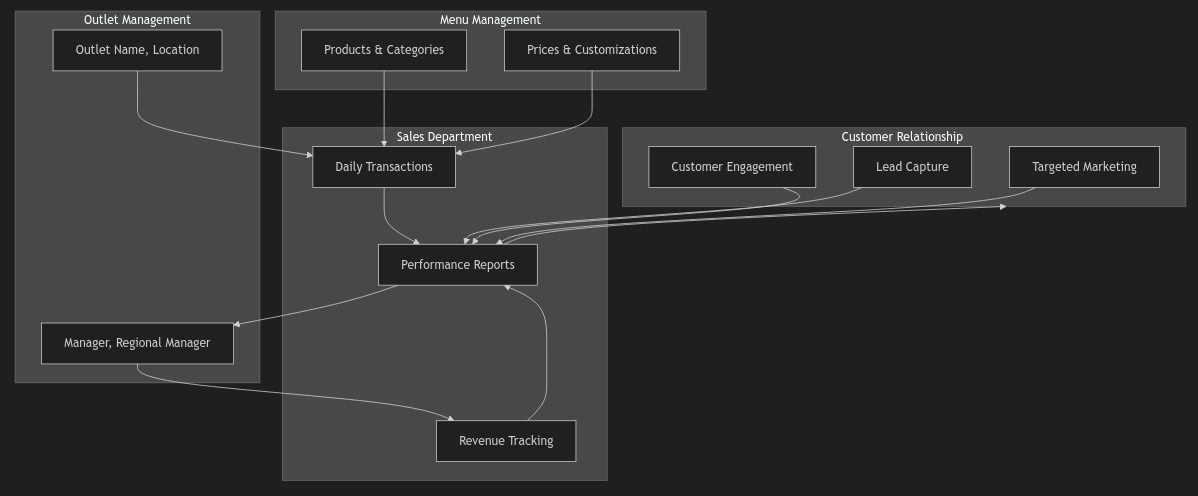
\includegraphics[width=0.9\textwidth,height=0.5\textheight,keepaspectratio]{diagrams/department.png}
\caption{Department Interaction Diagram of Coffee Chain ERP}
\end{figure}

\section*{Insights}
\begin{itemize}
    \item Departments are digitally connected, reducing fragmentation of data.  
    \item Centralization improves accuracy and ensures a single version of truth.  
    \item PDCA integration provides a cycle of continuous improvement.  
\end{itemize}

\chapter{SIPOC Analysis}

The SIPOC diagram provides a high-level overview of the Coffee Chain ERP process, highlighting how Suppliers, Inputs, Processes, Outputs, and Customers interact. It is a useful tool for understanding the flow of operations, identifying bottlenecks, and ensuring that all stakeholders’ needs are addressed.

\section*{Purpose of SIPOC}
The SIPOC framework helps us visualize the end-to-end process of the Coffee Chain ERP system. It allows management to:
\begin{itemize}
    \item Identify key suppliers and inputs required for smooth operations.
    \item Understand the critical processes that transform inputs into outputs.
    \item Ensure outputs meet the expectations of customers.
    \item Detect potential gaps or inefficiencies in the workflow.
\end{itemize}

\section*{Suppliers, Inputs, Processes, Outputs, Customers}

\subsection*{Suppliers}
\begin{itemize}
    \item \textbf{Coffee Outlets:} Provide sales data, menu updates, and operational feedback. They are the primary source of information for the ERP system.
    \item \textbf{Suppliers:} Supply raw ingredients, coffee beans, and other consumables. Timely delivery ensures smooth operations across outlets.
    \item \textbf{CRM:} Provides customer leads and engagement data, which is essential for marketing and sales tracking.
\end{itemize}

\subsection*{Inputs}
\begin{itemize}
    \item Product details, pricing, and menu configurations.
    \item Raw materials and stock updates from suppliers.
    \item Customer leads and engagement information from the CRM.
\end{itemize}

\subsection*{Processes}
\begin{itemize}
    \item Tracking daily sales and updating the ERP system.
    \item Managing product and menu updates in real-time.
    \item Receiving and logging stock from suppliers.
    \item Capturing customer interactions and monitoring CRM data.
\end{itemize}

\subsection*{Outputs}
\begin{itemize}
    \item Updated sales reports for each outlet and consolidated regional reports.
    \item Inventory reports and notifications for low-stock items.
    \item Real-time product updates for sales and POS systems.
    \item CRM insights for marketing and customer engagement.
\end{itemize}

\subsection*{Customers}
\begin{itemize}
    \item Management: Receives comprehensive reports for decision-making.
    \item Outlet Managers: Use outputs to manage day-to-day operations.
    \item Marketing/Sales Teams: Leverage CRM insights to plan campaigns.
    \item Customers: Benefit indirectly through accurate pricing, better product availability, and consistent service.
\end{itemize}

\section*{SIPOC Table}

\begin{table}[H]
\centering
\begin{tabular}{|p{3cm}|p{3cm}|p{4cm}|p{3cm}|p{3cm}|}
\hline
\textbf{Suppliers} & \textbf{Inputs} & \textbf{Process} & \textbf{Outputs} & \textbf{Customers} \\
\hline
Coffee outlets & Product & Track sales, update ERP, manage orders & Sales reports, product updates & Management, Customers \\
\hline
Suppliers & Ingredients, stock & Receive and log stock in ERP & Updated inventory & Outlet managers, Kitchen staff \\
\hline
CRM & Customer leads & Capture and manage leads & Lead reports, CRM data & Marketing, Sales team \\
\hline
\end{tabular}
\caption{SIPOC for Coffee Chain ERP}
\end{table}

\section*{Visual SIPOC Diagram}

\begin{figure}[H]
\centering
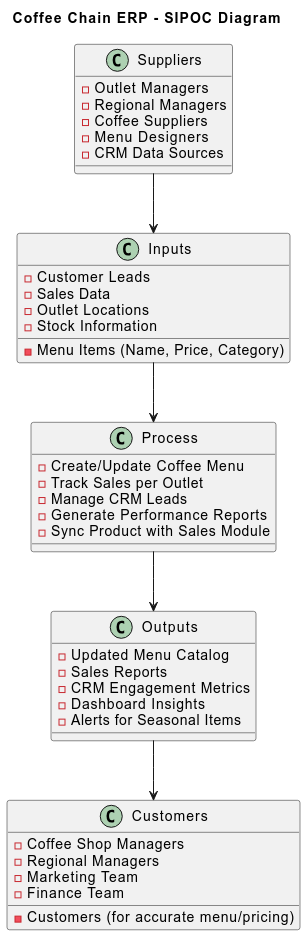
\includegraphics[width=0.85\textwidth,height=0.6\textheight,keepaspectratio]{diagrams/SIPOC.png}
\caption{Visual SIPOC Diagram of Coffee Chain ERP}
\end{figure}

\section*{Insights}
The SIPOC analysis highlights:
\begin{itemize}
    \item Critical dependency on real-time data from outlets and suppliers.
    \item Integration points between menu, sales, and CRM that require automated updates.
    \item The need for dashboards to provide management with actionable insights.
    \item Potential bottlenecks such as delayed supplier updates or manual sales entry.
\end{itemize}

\chapter{Module Role and Scope}

\section*{Role of the Coffee Chain ERP Module}

The Coffee Chain ERP module is designed to consolidate multiple business functions into a single, integrated platform. Its role is to streamline operations, improve data visibility, and provide actionable insights for decision-makers across the coffee outlet network. Specifically, the module serves the following purposes:

\begin{itemize}
    \item \textbf{Outlet Management:} Maintain records of outlet details such as name, location, assigned manager, and regional manager. This ensures consistent operational oversight across all outlets.
    \item \textbf{Sales Management:} Capture daily sales transactions, link sales with menu products, track revenue per outlet, and generate performance reports.
    \item \textbf{CRM Integration:} Manage customer leads, track interactions, and associate them with sales outcomes to enhance customer relationship management.
    \item \textbf{Menu Integration:} Administer coffee menu items, categories, and pricing, with automatic synchronization to the Sales module for real-time ordering.
    \item \textbf{Data Consolidation and Analytics:} Centralize information from multiple outlets for analysis, reporting, and decision-making.
\end{itemize}

\vspace{1em}

\section*{Scope}

The scope of the Coffee Chain ERP module defines its boundaries and functionalities:

\begin{itemize}
    \item Covers all active coffee outlets within the chain.
    \item Includes management of all menu items, product categories, and pricing.
    \item Captures daily sales transactions and integrates them with menu and CRM data.
    \item Provides real-time dashboards and reports for outlet managers and regional managers.
    \item Supports operational decision-making based on consolidated performance metrics.
    \item Excludes loyalty and reward management in the current version.
    \item Does not include outlet capacity tracking; operational staffing and space management are outside the current module scope.
\end{itemize}

\vspace{1em}

\section*{Stakeholders and KPIs}

The primary stakeholders and associated KPIs are outlined below:

\begin{itemize}
    \item \textbf{Outlet Managers:} Monitor outlet efficiency, daily revenue, and sales performance.  
          \textit{KPIs: revenue per outlet, sales per product, top-selling items.}
    \item \textbf{Regional Managers:} Compare performance across outlets within their region.  
          \textit{KPIs: total revenue, average sales per outlet, regional growth trends.}
    \item \textbf{Employees:} Ensure accurate data entry for sales, products, and customer interactions.  
          \textit{KPIs: transaction accuracy, product update consistency.}
    \item \textbf{Management and Decision-makers:} Access consolidated insights for strategic planning and operational improvements.  
          \textit{KPIs: lead conversion rate, overall revenue, sales growth trends.}
\end{itemize}

\vspace{1em}

\section*{Module Context Diagram (C1)}

The C1-Level Context Diagram illustrates the Coffee Chain ERP module, showing its interactions with key stakeholders, submodules (Outlet, Sales, Menu, CRM), and the flow of information between them.

\begin{figure}[H]
\centering
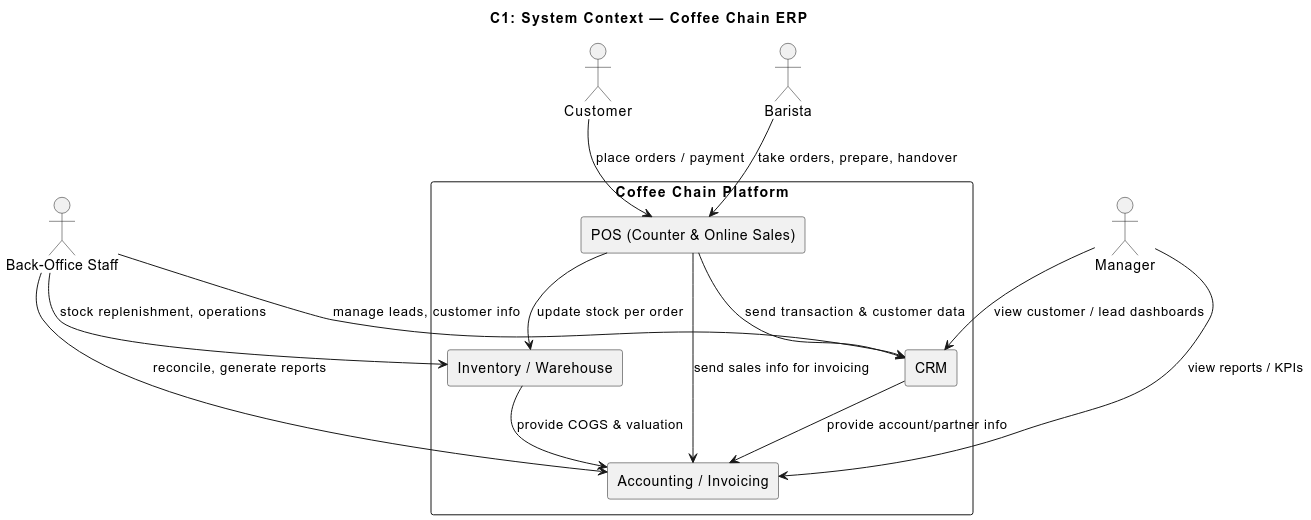
\includegraphics[width=0.9\textwidth,keepaspectratio]{diagrams/context.png}
\caption{C1-Level Context Diagram of Coffee Chain ERP}
\end{figure}

The diagram highlights how outlet data, sales transactions, menu updates, and CRM leads flow into the ERP system. Management and regional managers receive consolidated reports and insights. Each module interacts seamlessly to reduce manual work, ensure real-time synchronization, and improve decision-making.

\vspace{1em}

\section*{Insights}

\begin{itemize}
    \item The Coffee Chain ERP module centralizes multiple business functions, reducing operational fragmentation across outlets.
    \item Integration between Outlet, Sales, Menu, and CRM ensures real-time data synchronization, minimizing errors and manual updates.
    \item Consolidated dashboards and reporting empower managers and regional managers to make informed operational and strategic decisions.
    \item Linking menu items directly to sales products automates pricing updates and sales tracking, improving accuracy and efficiency.
    \item CRM integration enhances customer relationship management, allowing the business to track leads, improve engagement, and monitor conversion rates.
    \item The module provides a foundation for future expansions such as loyalty programs, outlet capacity tracking, or advanced analytics.
    \item By visualizing the system through the C1-Level Context Diagram, stakeholders can clearly understand interactions, responsibilities, and information flows.
    \item Overall, the ERP module streamlines multi-outlet operations, increases transparency, and strengthens decision-making capabilities across the coffee chain.
\end{itemize}

\chapter{Pain-Gain Canvas}

The Pain-Gain Canvas provides a structured overview of the challenges (Pains) faced by stakeholders in the Coffee Chain ERP system and the value additions (Gains) that the system delivers. It helps visualize how the ERP addresses critical operational pain points while creating tangible benefits for management, outlet staff, and customers.

\section*{Purpose of Pain-Gain Analysis}
The Pain-Gain Canvas helps stakeholders:
\begin{itemize}
    \item Identify key operational problems in the current workflow.
    \item Highlight the added value that the ERP system provides.
    \item Guide future enhancements and improvements for the ERP module.
    \item Align ERP functionality with organizational goals and user expectations.
\end{itemize}

\section*{Pains: Operational Challenges}

\begin{itemize}
    \item \textbf{Manual sales tracking across outlets:} Tracking sales individually in multiple locations is error-prone and time-consuming.
    \item \textbf{Menu updates not automatically reflected in sales:} Any changes in the coffee menu need to be manually synchronized with the sales module, leading to discrepancies.
    \item \textbf{Limited visibility into customer leads and engagement:} Without centralized CRM integration, marketing and sales teams lack actionable insights.
    \item \textbf{Difficulty generating consolidated reports:} Management cannot easily access regional or outlet-level performance data.
    \item \textbf{Data entry and pricing errors:} Manual processes increase the likelihood of mistakes affecting revenue.
    \item \textbf{Fragmented CRM data across outlets:} Leads and customer interactions are scattered, reducing the effectiveness of customer engagement strategies.
\end{itemize}

\section*{Gains: Value Additions}

\begin{itemize}
    \item \textbf{Centralized ERP platform:} Integrates outlets, sales, menu, and CRM into a single system for efficiency.
    \item \textbf{Real-time menu updates:} Ensures all sales channels reflect the latest product offerings immediately.
    \item \textbf{Automated reporting dashboards:} Provides management with comprehensive, actionable performance metrics for each outlet and region.
    \item \textbf{Enhanced decision-making:} Managers can make data-driven decisions with accurate and consolidated information.
    \item \textbf{Improved customer engagement:} Centralized CRM allows better tracking of leads and interactions across outlets.
    \item \textbf{Reduced errors via automation:} Minimizes mistakes in pricing, stock management, and sales tracking.
\end{itemize}

\section*{Visual Pain-Gain Canvas}

\begin{figure}[H]
\centering
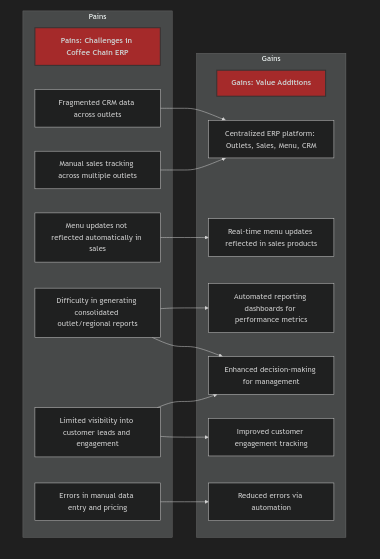
\includegraphics[width=0.85\textwidth,height=0.6\textheight,keepaspectratio]{diagrams/pain_gain.png}
\caption{Pain-Gain Canvas of Coffee Chain ERP}
\end{figure}

\section*{Insights}

\begin{itemize}
    \item The ERP system directly addresses the most critical operational challenges by centralizing processes.
    \item Automated menu updates and reporting dashboards are key features that convert operational pains into tangible gains.
    \item Customer engagement and sales tracking improvements ensure long-term value creation.
    \item The Pain-Gain Canvas serves as a guide for future ERP enhancements, highlighting areas for potential automation and integration.
    \item By addressing operational pains and leveraging system gains, the Coffee Chain ERP ensures:
    \begin{itemize}
        \item Smooth daily operations across all outlets.
        \item Real-time visibility into sales, menu, and CRM data.
        \item Improved decision-making at both outlet and regional levels.
        \item Enhanced customer satisfaction and business efficiency.
    \end{itemize}
\end{itemize}

\subsection*{Strategic Insight}

The Pain-Gain analysis also aligns directly with the Quality Management System (QMS) and the PDCA (Plan-Do-Check-Act) cycle described in Chapter 1.  
By addressing pains through ERP automation and integration, the system supports continuous improvement:

\begin{itemize}
    \item \textbf{Plan:} Identify operational inefficiencies such as manual sales tracking and fragmented CRM data.
    \item \textbf{Do:} Implement ERP features that centralize menu, sales, and CRM into a single platform.
    \item \textbf{Check:} Use automated reporting dashboards to monitor outlet performance, sales trends, and customer engagement.
    \item \textbf{Act:} Refine processes and update system configurations to enhance efficiency and customer satisfaction.
\end{itemize}

This demonstrates that the ERP not only resolves current pains but also creates a framework for sustainable, long-term improvements across the coffee chain.

\chapter{Components \& Containers}

This chapter provides a detailed breakdown of the Coffee Chain ERP system in terms of its \textbf{containers} (modules) and the internal \textbf{components} of each module. Understanding the containers and components is essential for grasping the system architecture and how different parts interact to achieve operational efficiency.

\section*{Definition of a Container}

In the context of Coffee Chain ERP, a \textbf{container} represents a deployable or executable part of the system, such as a web application, microservice, or database, that encapsulates a set of functionality. Containers can be thought of as the high-level building blocks of the system. For example, the Sales Module is a container because it is a standalone web application managing sales transactions, linked to menu and CRM modules.

\section*{Containers of Coffee Chain ERP (C2 Diagram)}

The following containers constitute the Coffee Chain ERP system:

\begin{itemize}
    \item \textbf{Outlet Management:} Web application managing outlet details, managers, and regional assignments.
    \item \textbf{Sales Module:} Web application capturing daily sales, linking products to orders, and generating performance reports.
    \item \textbf{CRM Module:} Web application tracking customer leads, interactions, and supporting targeted marketing.
    \item \textbf{Menu Module:} Web application managing products, categories, and prices, synchronized with Sales.
    \item \textbf{Reporting \& Analytics:} Web application providing dashboards and consolidated performance insights.
\end{itemize}

\begin{figure}[H]
\centering
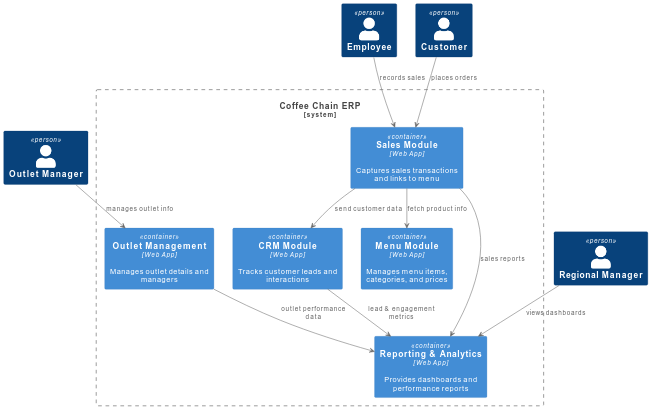
\includegraphics[width=0.9\textwidth,keepaspectratio]{diagrams/C2.png}
\caption{C2-Level Container Diagram of Coffee Chain ERP}
\end{figure}

\subsection*{Insights}

The C2 diagram illustrates how each module (container) interacts with other modules and external actors (employees, managers, customers). This high-level view helps stakeholders understand dependencies, system boundaries, and data flow without needing to inspect individual module internals.

\section*{Components of Each Container (C3 Diagrams)}

Each container is composed of internal components that define its functionality and interactions. These components are depicted in C3-level component diagrams.

\subsection*{Outlet Management Module Components}
\begin{itemize}
    \item Outlet Information Management
    \item Manager Assignment Component
    \item Regional Performance Component
    \item Reporting Component
\end{itemize}

\begin{figure}[H]
\centering
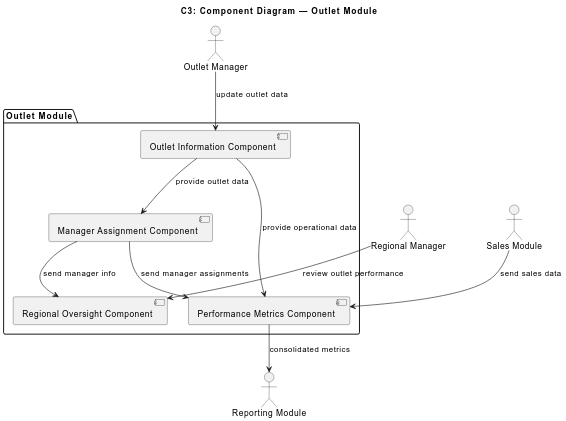
\includegraphics[width=0.9\textwidth,keepaspectratio]{diagrams/C3_outlet.png}
\caption{C3-Level Component Diagram — Outlet Management}
\end{figure}

\subsection*{Sales Module Components}
\begin{itemize}
    \item Transaction Processing Component
    \item Reporting Component
    \item Product Link Component
    \item Payment Processing Component
\end{itemize}

\begin{figure}[H]
\centering
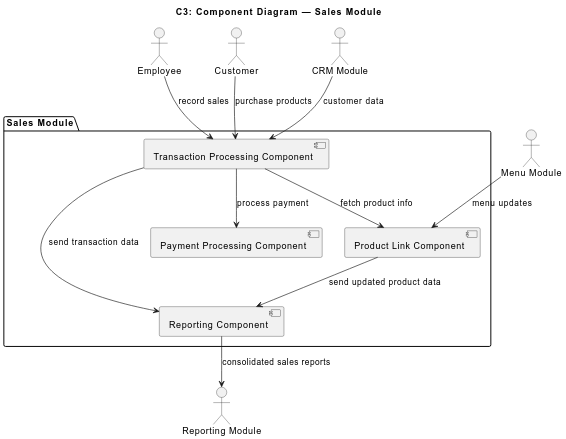
\includegraphics[width=0.9\textwidth,keepaspectratio]{diagrams/C3_sales.png}
\caption{C3-Level Component Diagram — Sales Module}
\end{figure}

\subsection*{CRM Module Components}
\begin{itemize}
    \item Lead Management Component
    \item Customer Interaction Component
    \item Customer Segmentation Component
    \item CRM Reporting Component
\end{itemize}

\begin{figure}[H]
\centering
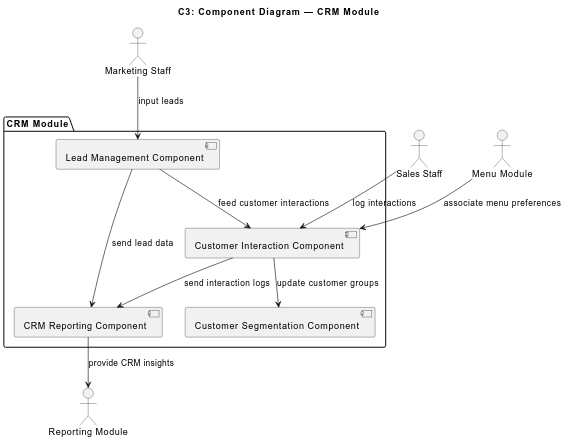
\includegraphics[width=0.9\textwidth,keepaspectratio]{diagrams/C3_crm.png}
\caption{C3-Level Component Diagram — CRM Module}
\end{figure}

\subsection*{Menu Module Components}
\begin{itemize}
    \item Menu Item Management Component
    \item Category Management Component
    \item Pricing Component
    \item Menu-Sales Synchronization Component
\end{itemize}

\begin{figure}[H]
\centering
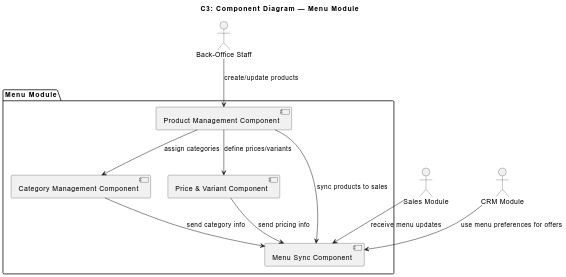
\includegraphics[width=0.9\textwidth,keepaspectratio]{diagrams/C3_menu.png}
\caption{C3-Level Component Diagram — Menu Module}
\end{figure}

\subsection*{Insights}

Analyzing the C3 diagrams reveals the following:

\begin{itemize}
    \item Each module has a clear separation of responsibilities via components.
    \item Internal components communicate with external actors (employees, customers, managers) and other modules to provide seamless operations.
    \item The ERP system’s modular architecture enables future extension, such as adding Loyalty \& Rewards or Inventory Management, without disrupting existing modules.
    \item Real-time synchronization between Menu, Sales, and CRM is critical for accurate reporting and decision-making.
\end{itemize}


\chapter{Components \& Integration}
\chapter{Concepts \& Documentation}

This chapter introduces the key concepts behind the Coffee Chain ERP system and details the important documents and records used in the workflow. Understanding these concepts is essential for grasping how the ERP operates and how data flows between modules.

\section*{Key Concepts}

\subsection*{1. ERP System Integration}
The Coffee Chain ERP is designed as an integrated platform combining multiple business functions—outlet management, sales, menu management, and CRM. Integration ensures that updates in one module automatically propagate to others, reducing manual work and errors.  

\textbf{Example:} Updating a menu item in the Menu module automatically updates the Sales module, ensuring that employees sell the correct items with accurate pricing.

\subsection*{2. Module-Based Architecture}
The ERP is organized into distinct modules (containers) and components:

\begin{itemize}
    \item \textbf{Outlet Management:} Stores information about each coffee outlet, including name, location, manager, and regional manager.
    \item \textbf{Sales Module:} Handles transactions, product linking, and performance reporting.
    \item \textbf{Menu Module:} Manages products, categories, and pricing, linking to the Sales module.
    \item \textbf{CRM Module:} Tracks customer leads, interactions, and engagement metrics.
    \item \textbf{Reporting \& Analytics:} Consolidates data from all modules for dashboards and decision support.
\end{itemize}

\subsection*{3. Workflow Concepts}
\begin{itemize}
    \item \textbf{Transaction Flow:} From order placement to sales recording, each step is logged in the ERP for accuracy.
    \item \textbf{Data Synchronization:} Changes in one module (e.g., menu updates) reflect immediately in dependent modules (e.g., sales).
    \item \textbf{Decision Support:} Consolidated reports allow managers and regional managers to track KPIs such as revenue, product sales, and lead conversion rates.
\end{itemize}

\subsection*{4. User Roles and Responsibilities}
\begin{itemize}
    \item \textbf{Outlet Managers:} Manage outlet operations and ensure accurate data entry.
    \item \textbf{Regional Managers:} Compare performance across outlets and make strategic decisions.
    \item \textbf{Employees:} Enter sales and product information accurately.
    \item \textbf{Customers:} Interact with the system via orders; indirectly feed CRM data.
\end{itemize}

\subsection*{5. Concept of Containers and Components}
In this ERP context:
\begin{itemize}
    \item A \textbf{Container} represents a high-level module such as Sales, CRM, or Menu.
    \item A \textbf{Component} is a sub-part of a container that executes a specific function, e.g., the \emph{Transaction Processing Component} in Sales.
\end{itemize}

\section*{Documents in the Workflow}

\subsection*{1. Sales Records}
\begin{itemize}
    \item Captured automatically by the Sales module.
    \item Includes transaction ID, product sold, quantity, price, payment method, and timestamp.
    \item Serves as the basis for financial reports and performance analytics.
\end{itemize}

\subsection*{2. Menu Master List}
\begin{itemize}
    \item Contains all products, categories, and pricing information.
    \item Maintained in the Menu module; synchronized with Sales.
    \item Provides consistency in product offerings across outlets.
\end{itemize}

\subsection*{3. Customer \& Lead Records}
\begin{itemize}
    \item Captured by the CRM module.
    \item Includes lead source, customer information, interaction logs, and engagement metrics.
    \item Used for marketing, promotions, and improving customer relationships.
\end{itemize}

\subsection*{4. Outlet Data Sheets}
\begin{itemize}
    \item Contains outlet details: name, location, manager, regional manager.
    \item Maintained in the Outlet Management module.
    \item Supports reporting and operational oversight.
\end{itemize}

\subsection*{5. Reports and Dashboards}
\begin{itemize}
    \item Generated by the Reporting \& Analytics module.
    \item Summarizes sales, outlet performance, and customer engagement.
    \item Provides actionable insights for decision-making.
\end{itemize}

\section*{Integration of Documents with Modules}

\begin{itemize}
    \item Sales records are linked to menu items and CRM leads.
    \item Customer engagement documents feed into reporting dashboards.
    \item Outlet data is referenced for KPI calculation and performance benchmarking.
\end{itemize}

\section*{Code and Diagram Integration}

\begin{lstlisting}[language=Python, caption={Example: Sales Transaction Recording in Python}]
class SaleOrder(models.Model):
    _inherit = 'sale.order'

    outlet_id = fields.Many2one('coffee.outlet', string='Outlet')
    customer_id = fields.Many2one('res.partner', string='Customer')
\end{lstlisting}

\begin{figure}[H]
\centering
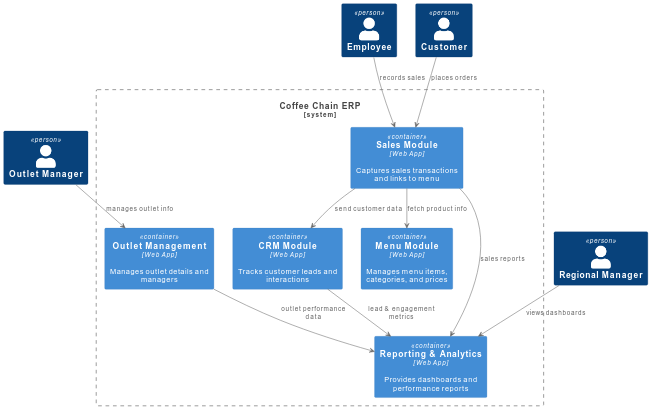
\includegraphics[width=0.9\textwidth,keepaspectratio]{diagrams/C2.png}
\caption{Reference Container Diagram for Document Flow}
\end{figure}

\section*{Insights}

\begin{itemize}
    \item Centralizing document management reduces errors and ensures data consistency.
    \item Clear linkage between documents and modules enhances traceability and decision-making.
    \item Automated capture of sales, menu, and customer data minimizes manual intervention.
    \item Reporting dashboards serve as the single source of truth for management insights.
\end{itemize}

\chapter{Workflow and Customer Journey for Coffee Chain ERP System}

\section*{Introduction}
This chapter describes the workflow and customer journey in the Coffee Chain ERP system. The system is designed to manage coffee outlets, menu items, sales orders, and customer information. The goal is to provide a clear understanding of how users (staff and administrators) interact with the system and how sale customers experience the ordering process.

\section*{System Entities}
The main entities in the Coffee Chain ERP system are:

\begin{itemize}
    \item \textbf{Coffee Outlet (\texttt{coffee.outlet})}: Represents a coffee outlet in the chain.
    \item \textbf{Outlet Owner (\texttt{res.partner})}: Represents the owner of a coffee outlet.
    \item \textbf{Coffee Menu Item (\texttt{coffee.menu.item})}: Represents drinks and snacks available for order.
    \item \textbf{Sale Customer (\texttt{res.partner})}: Represents the end customer purchasing products at the outlet.
    \item \textbf{Sale Order (\texttt{sale.order})}: Represents a customer's order in the system.
    \item \textbf{CRM Lead (\texttt{crm.lead})}: Optional linkage for sales leads and customer management.
\end{itemize}

\section*{Workflow Sequence}
The workflow represents the operations performed by administrators and staff for managing outlets, menu items, customers, and sales orders.

\subsection*{Administrator Workflow}
Administrators are responsible for setting up outlets, outlet owners, and menu items. The workflow is as follows:

\begin{enumerate}
    \item Create or manage \textbf{Outlet Owner} (\texttt{res.partner}).
    \item Create or view a \textbf{Coffee Outlet} and assign it to an outlet owner.
    \item Create \textbf{Menu Items} (drinks and snacks) that can later be added to customer orders.
    \item Create or manage \textbf{Sale Customers} (\texttt{res.partner}) who purchase items at the outlet.
    \item Optionally link \textbf{CRM Leads} to track customer interactions.
\end{enumerate}

\begin{figure}[H]
    \centering
    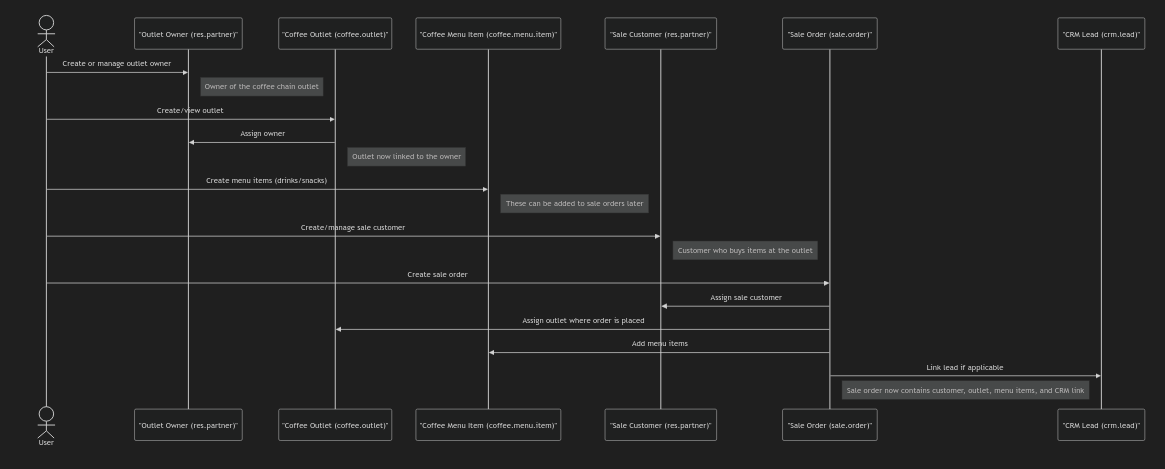
\includegraphics[width=0.85\textwidth]{diagrams/sequence.png}
    \caption{Administrator Workflow Sequence Diagram}
\end{figure}

\section*{Customer Journey}
The customer journey demonstrates how a sale customer interacts with the coffee outlet via the staff (barista) using the POS system.

\subsection*{Steps in the Customer Journey}
\begin{enumerate}
    \item Customer approaches the outlet and places an order with the staff.
    \item Staff identifies the outlet where the order is being placed.
    \item Staff adds the selected menu items to a \textbf{Sale Order}.
    \item Sale order is linked to the outlet and optionally to a CRM lead.
    \item Customer makes payment to the staff.
    \item Staff confirms the order and issues a receipt.
    \item Sale is recorded in the system, including customer details, menu items, outlet, and CRM link if applicable.
\end{enumerate}

\begin{figure}[H]
    \centering
    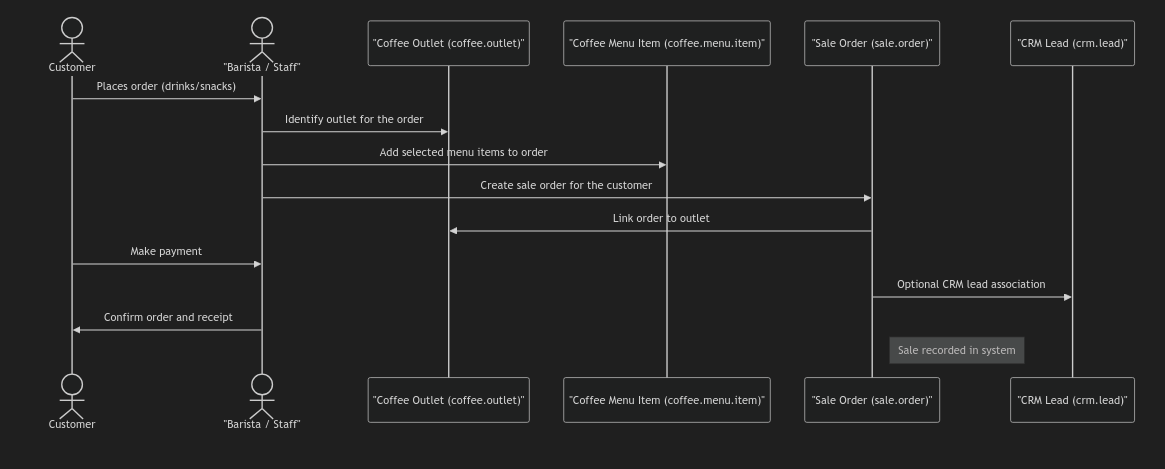
\includegraphics[width=0.85\textwidth]{diagrams/customer_journey.png}
    \caption{Customer Journey Sequence Diagram}
\end{figure}


This chapter provided a detailed workflow and customer journey for the Coffee Chain ERP system. By separating the \textbf{administrator workflow} from the \textbf{customer journey}, the system clearly defines responsibilities and interactions:

\begin{itemize}
    \item Administrators manage outlets, owners, and menu items.
    \item Staff (baristas) enter orders and process payments on behalf of customers.
    \item Sale orders record all interactions with outlets, menu items, customers, and optionally CRM leads.
\end{itemize}


\chapter{Code, Class, and Master Data Schema for Coffee Chain ERP System}

\section*{Introduction}
This chapter explains the master data structure and schema used in the Coffee Chain ERP system. It first introduces key terminologies for understanding ERP data models, then describes the master data entities, relationships, and schema as implemented in the system. This provides a foundation for understanding the system’s code and database structure.

\section*{Basic Terminologies}

\begin{description}
    \item[Entity:] A distinct object or concept in the system that stores data. Examples include Customer, Product, or Outlet.
    \item[Attribute:] A property or field of an entity. For example, a Customer entity may have attributes such as Name, Email, and Phone Number.
    \item[Primary Key:] A unique identifier for an entity instance. In Odoo, this is often the \texttt{id} field.
    \item[Relationship:] The association between two entities, such as One-to-Many or Many-to-One. Example: Each Outlet is owned by one Outlet Owner, while an owner can have multiple outlets.
    \item[Master Data:] Core data that is essential for the operation of a system, such as Customers, Products, and Outlets.
    \item[Business Logic Layer:] Code that defines the rules and behavior of the system, often implemented via Python classes in Odoo modules.
    \item[Model/Class:] In Odoo, a model is a Python class that defines the structure of an entity, including fields, relationships, and methods.
\end{description}

\section*{Master Data in Coffee Chain ERP System}
The Coffee Chain ERP system’s master data schema includes the following key entities:

\subsection*{Outlet Owner (\texttt{res.partner})}
\begin{tabular}{|l|l|l|}
\hline
\textbf{Field} & \textbf{Type} & \textbf{Description} \\
\hline
id & int & Primary Key \\
name & string & Owner Name \\
email & string & Contact Email \\
phone & string & Contact Number \\
\hline
\end{tabular}

\noindent
\textbf{Relationship:} One owner can manage multiple Coffee Outlets (One-to-Many).

\subsection*{Coffee Outlet (\texttt{coffee.outlet})}
\begin{tabular}{|l|l|l|l|}
\hline
\textbf{Field} & \textbf{Type} & \textbf{Description} & \textbf{Relationship} \\
\hline
id & int & Primary Key & — \\
name & string & Outlet Name & — \\
location & string & Outlet Address & — \\
owner\_id & int & Foreign Key & res.partner.id (Outlet Owner) \\
\hline
\end{tabular}

\noindent
\textbf{Relationships:} Many-to-One with Outlet Owner, One-to-Many with Sale Orders.

\subsection*{Coffee Menu Item (\texttt{coffee.menu.item})}
\begin{tabular}{|l|l|l|}
\hline
\textbf{Field} & \textbf{Type} & \textbf{Description} \\
\hline
id & int & Primary Key \\
name & string & Item Name \\
price & float & Item Price \\
category & selection & Drinks / Snacks \\
image & binary & Item Image \\
\hline
\end{tabular}

\noindent
\textbf{Relationship:} Many-to-Many with Sale Orders.

\subsection*{Sale Customer (\texttt{res.partner})}
\begin{tabular}{|l|l|l|}
\hline
\textbf{Field} & \textbf{Type} & \textbf{Description} \\
\hline
id & int & Primary Key \\
name & string & Customer Name \\
email & string & Contact Email \\
phone & string & Contact Number \\
\hline
\end{tabular}

\noindent
\textbf{Relationship:} One-to-Many with Sale Orders; optional link to CRM Leads.

\subsection*{Sale Order (\texttt{sale.order})}
\begin{tabular}{|l|l|l|l|}
\hline
\textbf{Field} & \textbf{Type} & \textbf{Description} & \textbf{Relationship} \\
\hline
id & int & Primary Key & — \\
order\_number & string & Unique Order Number & --- \\
customer\_id & int & Foreign Key & res.partner.id (Sale Customer) \\
outlet\_id & int & Foreign Key & coffee.outlet.id \\
order\_date & date & Order Timestamp & --- \\
\hline
\end{tabular}

\noindent
\textbf{Relationship:} Many-to-One with Sale Customer and Outlet; Many-to-Many with Menu Items; optional FK to CRM Lead.

\subsection*{CRM Lead (\texttt{crm.lead})}
\begin{tabular}{|l|l|l|l|}
\hline
\textbf{Field} & \textbf{Type} & \textbf{Description} & \textbf{Relationship} \\
\hline
id & int & Primary Key & — \\
lead\_name & string & Lead Title & --- \\
stage & string & Lead Status & — \\
related\_order\_id & int & Optional FK & sale.order.id \\
\hline
\end{tabular}

\noindent
\textbf{Relationship:} Optional linkage to Sale Orders and Sale Customers.

\section*{Master Data Schema Diagram}
The following diagram visually represents the **tables, fields, primary keys, and relationships** in the Coffee Chain ERP system:

%\begin{figure}[H]
 %   \centering
  %  \includegraphics[width=0.9\textwidth]{diagrams/masterdata_schema.png}
   % \caption{Master Data Schema showing entities, attributes, primary keys, and relationships.}
%\end{figure}

\section*{Python Classes Mapping to Master Data}
The ERP system implements the master data entities as Python classes in Odoo modules:

\begin{itemize}
    \item \texttt{coffee.outlet} → Python class \texttt{CoffeeOutlet(models.Model)}
    \item \texttt{coffee.menu.item} → Python class \texttt{CoffeeMenuItem(models.Model)}
    \item \texttt{res.partner} → Used for both Outlet Owner and Sale Customer
    \item \texttt{sale.order} → Python class \texttt{SaleOrder(models.Model)}
    \item \texttt{crm.lead} → Python class \texttt{CrmLead(models.Model)}
\end{itemize}

\subsection*{Field Definitions Example}
For example, the \texttt{CoffeeMenuItem} class defines the following fields:

\begin{lstlisting}[language=Python, caption={Coffee Menu Item Python Class}]
from odoo import models, fields

class CoffeeMenuItem(models.Model):
    _name = 'coffee.menu.item'
    _description = 'Coffee Menu Item'

    name = fields.Char(required=True)
    price = fields.Monetary(currency_field='currency_id', required=True)
    category = fields.Selection([
        ('drinks', 'Drinks'),
        ('snacks', 'Snacks'),
    ], required=True)
    image = fields.Image(max_width=128, max_height=128)
\end{lstlisting}

\begin{figure}[H]
    \centering
    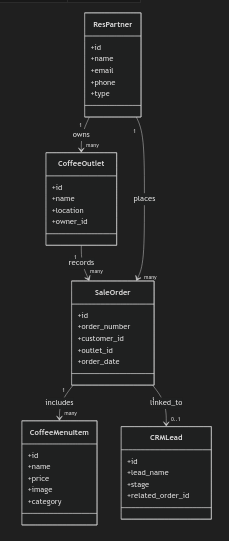
\includegraphics[width=0.356\textwidth]{diagrams/masterdata.png}
    \caption{Class diagram showing Python classes and field names for quick reference.}
\end{figure}

\section*{Summary}
The master data schema of the Coffee Chain ERP system ensures:

\begin{itemize}
    \item Clear separation of entities: outlets, menu items, customers, orders, and leads.
    \item Proper relationships to maintain data integrity: e.g., orders linked to customers and outlets.
    \item Python classes in Odoo accurately define the structure, fields, and relationships.
    \item The schema supports the business logic and workflow described in previous chapters.
\end{itemize}

\chapter{Access Rights and User Roles in Coffee Chain ERP System}

\section*{Introduction}
Access control is a fundamental aspect of any ERP system. It ensures that users can only access data and perform actions according to their responsibilities. This chapter explains the concept of access rights, user roles, and how they are implemented in Odoo. Finally, it details the specific access rights configured for the Coffee Chain ERP system based on its code.

\section*{General Concepts: Access Rights and User Roles}
\begin{description}
    \item[Access Rights:] Define what operations a user can perform on data. These typically include:
        \begin{itemize}
            \item \textbf{Read:} View records.
            \item \textbf{Write:} Edit existing records.
            \item \textbf{Create:} Add new records.
            \item \textbf{Delete / Unlink:} Remove records.
        \end{itemize}
    \item[User Roles:] Groupings of users with similar responsibilities. A role determines which models and actions a user can access.
    \item[Role-Based Access Control (RBAC):] Common model where access is granted based on the user’s role rather than individual permissions.
\end{description}


\section*{Access Control in Odoo}
In Odoo, access rights are managed using:
\begin{itemize}
    \item \textbf{Groups:} Collections of users sharing the same role.
    \item \textbf{Models:} Entities like \texttt{res.partner}, \texttt{sale.order}, or \texttt{coffee.menu.item}.
    \item \textbf{Permissions:} Defined in \texttt{ir.model.access.csv}, specifying read, write, create, and delete rights for a group on a model.
\end{itemize}

Each record operation in Odoo checks:
\begin{enumerate}
    \item Whether the user belongs to a group with the necessary permission.
    \item Whether the record is accessible under record rules (not covered in this chapter but relevant for finer control).
\end{enumerate}

\section*{User Roles in Coffee Chain ERP System}
The Coffee Chain ERP system defines the following primary user roles:

\begin{itemize}
    \item \textbf{Outlet User:} Staff who manage outlet operations, including sales orders, POS transactions, accounting entries, and menu items.
    \item \textbf{CRM User:} Staff who manage CRM leads and related customer interactions.
    \item \textbf{Help User:} Users who only need read access to help documents and guides.
\end{itemize}

These roles are implemented in Odoo using groups such as \texttt{base.group.user} and custom groups defined in the modules.

\section*{Access Rights for Coffee Chain ERP System}
The following table presents a matrix of access rights for the models in the system, derived from the \texttt{ir.model.access.csv} files in the modules:

% Table 1: ID, Name, Model
\begin{table}[H]
\centering
\begin{tabular}{|p{6cm}|p{6cm}|p{5cm}|}
\hline
\textbf{ID} & \textbf{Name} & \textbf{Model} \\
\hline
access\_coffee\_outlet\_user & access.coffee.outlet.user & coffee.outlet \\
access\_crm\_lead\_inherit\_user & access.crm.lead.inherit.user & crm.lead \\
access\_res\_partner\_inherit\_user & access.res.partner.inherit.user & res.partner \\
access\_coffee\_help\_user & access.coffee.help.user & coffee.help \\
access\_coffee\_crm\_help\_user & access.coffee.crm.help.user & coffee.crm.help \\
access\_coffee\_sales\_help\_user & access.coffee.sales.help.user & coffee.sales.help \\
access\_sale\_order\_outlet\_user & access.sale.order.outlet.user & sale.order \\
access\_sale\_order\_line\_coffee\_user & access.sale.order.line.coffee.user & sale.order.line \\
access\_account\_move\_outlet\_user & access.account.move.outlet.user & account.move \\
access\_account\_payment\_outlet\_user & access.account.payment.outlet.user & account.payment \\
access\_pos\_config\_outlet & access.pos.config.outlet & pos.config \\
access\_pos\_order\_outlet\_user & access.pos.order.outlet.user & pos.order \\
access\_pos\_order\_line\_outlet\_user & access.pos.order.line.outlet.user & pos.order.line \\
access\_coffee\_menu\_item\_user & access.coffee.menu.item & coffee.menu.item \\
access\_coffee\_menu\_tag\_user & access.coffee.menu.tag & coffee.menu.tag \\
\hline
\end{tabular}

\end{table}

% Table 2: Model continuation
\begin{table}[H]
\centering
\begin{tabular}{|p{5cm}|p{4cm}|c|c|c|c|c|}
\hline
\textbf{Model} & \textbf{Group} & \textbf{Read} & \textbf{Write} & \textbf{Create} & \textbf{Delete} \\
\hline
coffee.outlet & base.group.user & 1 & 1 & 1 & 1 \\
crm.lead & base.group.user & 1 & 1 & 1 & 1 \\
res.partner & base.group.user & 1 & 1 & 1 & 1 \\
coffee.help & — & 1 & 0 & 0 & 0 \\
coffee.crm.help & — & 1 & 0 & 0 & 0 \\
coffee.sales.help & — & 1 & 0 & 0 & 0 \\
sale.order & — & 1 & 1 & 1 & 1 \\
sale.order.line & — & 1 & 1 & 1 & 1 \\
account.move & — & 1 & 1 & 1 & 1 \\
account.payment & — & 1 & 1 & 1 & 1 \\
pos.config & base.group.user & 1 & 1 & 0 & 0 \\
pos.order & base.group.user & 1 & 1 & 1 & 1 \\
pos.order.line & base.group.user & 1 & 1 & 1 & 1 \\
coffee.menu.item & — & 1 & 1 & 1 & 1 \\
coffee.menu.tag & — & 1 & 1 & 1 & 1 \\
\hline
\end{tabular}
\caption{User Access Rights Matrix for Coffee Chain ERP System}
\end{table}




\section*{Explanation of Key Permissions}
\begin{itemize}
    \item Outlet-related models (\texttt{coffee.outlet}, \texttt{sale.order}, \texttt{pos.order}, etc.) have full CRUD access for staff responsible for operations.
    \item CRM models (\texttt{crm.lead}) allow full management for CRM users.
    \item Help-related models (\texttt{coffee.help}, \texttt{coffee.crm.help}, \texttt{coffee.sales.help}) are read-only to prevent modification by general users.
    \item POS configuration (\texttt{pos.config}) is restricted from creation to avoid accidental setups.
    \item Coffee menu items and tags can be fully managed by outlet staff to ensure menu updates.
\end{itemize}

\section*{Practical Examples of Access Control}

To better illustrate how access rights operate in practice:

\begin{itemize}
    \item A \textbf{regional manager} can view performance reports for multiple outlets but cannot directly edit outlet menus or prices. This ensures visibility without risking accidental changes to operational data.
    \item An \textbf{employee} (e.g., barista) can create sales orders and process transactions in the POS system but cannot modify outlet profiles or assign outlet managers. This limits their permissions to day-to-day operational tasks only.
    \item A \textbf{CRM user} can manage leads and customer interactions but cannot delete accounting entries or modify sales orders, keeping financial data protected.
\end{itemize}

These examples show how the system enforces the principle of least privilege, ensuring that each role has exactly the access needed to perform its duties, no more and no less.


This chapter explains general concepts of access rights and user roles, how they are implemented in Odoo, and the specific permissions configured for the Coffee Chain ERP system. The matrix provides a clear reference for developers, system administrators, and auditors to understand role-based access control within the system.

\end{document}
